 %%%%%%%%%%%%%%%%%%%%%%%%%%%%%%%%%%%%%%%%%
% Stylish Article
% LaTeX Template
% Version 2.2 (2020-10-22)
%
% This template has been downloaded from:
% http://www.LaTeXTemplates.com
%
% Original author:
% Mathias Legrand (legrand.mathias@gmail.com)
% With extensive modifications by:
% Vel (vel@latextemplates.com)
%
% License:
% CC BY-NC-SA 3.0 (http://creativecommons.org/licenses/by-nc-sa/3.0/)
%
%%%%%%%%%%%%%%%%%%%%%%%%%%%%%%%%%%%%%%%%%

%----------------------------------------------------------------------------------------
%	PACKAGES AND OTHER DOCUMENT CONFIGURATIONS
%----------------------------------------------------------------------------------------

\documentclass[10pt]{SelfArx} % Document font size and equations flushed left

\usepackage[english]{babel} % Specify a different language here - english by default
\usepackage{pgfgantt}

\usepackage{lipsum} % Required to insert dummy text. To be removed otherwise

\usepackage{rotating}

\newcommand{\beginsupplement}{%
        \setcounter{table}{0}
        \renewcommand{\thetable}{S\arabic{table}}%
        \setcounter{figure}{0}
        \renewcommand{\thefigure}{S\arabic{figure}}%
     }
%----------------------------------------------------------------------------------------
%	COLUMNS
%----------------------------------------------------------------------------------------

\setlength{\columnsep}{0.55cm} % Distance between the two columns of text
\setlength{\fboxrule}{0.75pt} % Width of the border around the abstract

%----------------------------------------------------------------------------------------
%	COLORS
%----------------------------------------------------------------------------------------

\definecolor{color1}{RGB}{0,0,90} % Color of the article title and sections
\definecolor{color2}{RGB}{0,20,20} % Color of the boxes behind the abstract and headings

%----------------------------------------------------------------------------------------
%	HYPERLINKS
%----------------------------------------------------------------------------------------

\usepackage{hyperref} % Required for hyperlinks

\usepackage{float}
\usepackage{makecell}
\hypersetup{
	hidelinks,
	colorlinks,
	breaklinks=true,
	urlcolor=color2,
	citecolor=color1,
	linkcolor=color1,
	bookmarksopen=false,
	pdftitle={Title},
	pdfauthor={Author},
}
\usepackage{multicol}
\usepackage{float}

%----------------------------------------------------------------------------------------
%	ARTICLE INFORMATION
%----------------------------------------------------------------------------------------

\JournalInfo{Laboratory of biological data mining} % Journal information
\Archive{Project outline} % Additional notes (e.g. copyright, DOI, review/research article)

\PaperTitle{Medulloblastoma: Human Specific Genes Contribution} % Article title

\Authors{Sara Baldinelli, Letizia De Pietri, Gaia Faggin, Huyen Pham, Roan Spadazzi} % Authors

\Keywords{} % Keywords - if you don't want any simply remove all the text between the curly brackets
\newcommand{\keywordname}{Keywords} % Defines the keywords heading name

%----------------------------------------------------------------------------------------
%	ABSTRACT
%----------------------------------------------------------------------------------------

\Abstract{Medulloblastoma (MB) is the most prevalent malignant brain tumor in childhood. It poses a significant health challenge and impacts children at a rate tenfold higher than adults. The disease is molecularly heterogeneous, with distinct subgroups (MB-WNT, SHH, Gp3, and Gp4) exhibiting variations in cytogenetics, mutational profiles, and gene expression signatures, shaping treatment strategies and outcomes. Since the disease origins are primarily genomic alterations, we aim to investigate if the MB driving genes are also Human Specific Genes (HSGs). As HSGs are unique to humans, they often underpin distinctive traits that evolved recently or undergo significant changes. As a result, they often play critical roles in brain functions, immune systems, and metabolic processes. Our research seeks to identify MB HSGs, their function and their potential for being bio-markers and drug targets. We will integrate the set of MB-associated HSGs with FANTOM causal relations and perform functional and network analyses on the resultant gene set. Our findings will lead to further investigation on the biological development of the disease, that may offer valuable insights into its evolution and implications for targeted therapies or treatment strategies.}
%----------------------------------------------------------------------------------------

\begin{document}

\maketitle % Output the title and abstract box
%\tableofcontents % Output the contents section

%\thispagestyle{empty} % Removes page numbering from the first page

%----------------------------------------------------------------------------------------
%	ARTICLE CONTENTS
%----------------------------------------------------------------------------------------

\section*{Introduction}\label{sec:introduction}
Medulloblastoma (MB) stands as the most prevalent malignant brain tumor in childhood, constituting roughly 20\% of pediatric central nervous system tumors \cite{kumar2017challenges}, and impacting children at a rate tenfold higher than adults \cite{carta2020cancer}. This condition is categorized into distinct molecular subgroups: MB-WNT, Sonic Hedgehog (SHH), Group 3 (Gp3) and Group 4 (Gp4). These subgroups exhibit striking differences in cytogenetics, mutational profiles, and gene expression signatures, all of which significantly influence the treatment strategies and outcomes \cite{chen2022molecular}. \\
Given its prevalence in childhood, MB's origins cannot be attributed to environmental or age-related factors. Instead, it is primary driven by genomic alterations. \\
Previous studies showed that the least to most common sub-groups are: WNT, Group 3, SHH and Group 4. Respectively, they have survival rates of: $\sim$95\%, $\sim$50\%, $\sim$60-80\% and, $\sim$75\%. \cite{northcott2012medulloblastomics, hovestadt2020medulloblastomics}.\\
In our project we will investigate the contribution of Human Specific Genes (HSGs) with respect to non-HSGs in the context of this disease. \\
HSGs are genes that are unique to the human species and have no direct counterparts in the genome of other closely related species, such as our primate relatives. These genes are often considered to be responsible for traits or functions that are distinctive to humans; they may have evolved relatively recently in the human lineage or have undergone significant changes that make them distinct from the genes found in other species. Identification and study of HSGs could provide insight into what sets humans apart from other species. \\ 
It is worth noting that a substantial portion of HSGs plays a critical role in brain functions, alongside their roles in the immune system and metabolic processes \cite{bitar2019genes}.\\
Consequently, our efforts are directed towards identifying HSGs that may contribute to the development of MB. \\
To this purpose, the set of MB HSGs will be integrated with FANTOM \cite{fantom5} causal relations. A functional and a network analysis will be carried out on the resulting set of genes and hypotheses about the role of HSGs in the context of MB will be formulated based on the results. \\

\section{Biological question}\label{sec:biological_question}
The question driving this project revolves around the role of Human Specific Genes in comparison to non-HSGs within the context of MB. \\
In order to address this question, we will assess the following points: 
\begin{enumerate}
    \item Identifying the existence of causal relationships among HSGs specific to MB and elucidating their significance. 
    \item Evaluating the functional significance of the subset of HSGs associated with MB.
    \item Investigating the network structure constructed from the subset of HSGs. 
\end{enumerate}
Collectively, these objectives will help us to acquire the knowledge necessary to uncover the significance of HSGs in MB and determine the level at which these genes can serve as markers for subtyping MB.

\section{Data}\label{sec:data}

\subsection{Cohort selection}\label{sec:cohort_selection}

\subsubsection{GSE155446}\label{sec:GSE155446}
Cohort GSE155446 \cite{riemondy2022neoplastic} represents a comprehensive exploration of cellular heterogeneity within 28 childhood MB cases, classified into different subgroups, including 1 WNT, 9 SHH, 7 Gp3 and 11 Gp4 MB. \\
This study investigates cellular diversity in childhood MB using single-cell RNA sequencing, revealing distinct neoplastic cell subpopulations associated with mitotic, undifferentiated and neuronal profiles. 

\subsection{List of Human Specific Genes}\label{sec:list_genes}
A list of 856 genes specific to humans was extracted from the research conducted by Bitar et al. \cite{bitar2019genes}. This list will serve as a reference for pinpointing HSGs among the set of genes retrieved. \\

\subsection{FANTOM dataset}\label{sec:Fantom_dataset}
The FANTOM \cite{fantom5} dataset will be used to expand the set of MB HSGs so that genes involved in causal relations will also be considered.

\section{Pipeline}\label{sec:pipeline}
The project workflow is described in \textbf{Figure \ref{fig:workflow}}. Following it, it is possible to divide the work in six main steps.

\begin{enumerate}
    \item Data pre-processing;
    \item Differential expression analysis; 
    \item Intersection between MB differentially expressed genes and the list of Human Specific Genes;
    \item Data integration between the filtered MB Human Specific Genes and the FANTOM data;
    \item Functional Analysis;
    \item Network Analysis.
\end{enumerate}

\subsection{Data pre-processing}\label{sec:pre_processing}
In our project, we will leverage the power of \textit{Scanpy} \cite{wolf2018scanpy} to conduct data pre-processing for scRNA-seq datasets, a crucial initial step in our analysis pipeline. This pre-processing workflow is pivotal for handling the complexity of scRNA-seq data and ensuring the accuracy of downstream analyses. We will begin by importing the raw count matrix into \textit{Scanpy}'s AnnData object, facilitating data organization and management. Quality control will follow, where we will apply stringent filters to eliminate low-quality cells and genes based on criteria such as minimum count per cell or gene expression levels. To reduce technical bias, we will normalize the data using library size scaling or log transformation. For dimensionality reduction, techniques like PCA or UMAP will be employed to uncover the underlying structure of the data. Clustering algorithms will help identifying distinct cell populations, and marker genes will be detected to label cell types accurately. \\

\subsection{Differential expression analysis}
Following the initial data pre-processing steps, the next crucial phase involves conducting differential expression analysis. This process is a fundamental component of scRNA-seq data analysis and it plays a key role in the identification of genes that exhibit significant unpregulation or downregulation within a specific cell population, under various conditions or in response to distinct treatments. \\
To accomplish this task, we will also use, during this step, the \textit{Scanpy} library \cite{wolf2018scanpy}.

\subsection{Intersection between MB differentially expressed genes and the list of Human Specific Genes}
After obtaining our differentially expressed genes, we will intersect them with the list of Human Specific Genes.  

\subsection{Integrate the filtered MB Human Specific Genes with the FANTOM data}
After obtaining our list of HSGs related to MB, we will integrate them with the FANTOM \cite{fantom5} dataset in order to retrieve causal relations.

\subsection{Functional Analysis}\label{sec:functional_analysis}
Functional analysis involves leveraging various bioinformatics tools and databases such as Gene Ontology (GO) \cite{gene2019gene} enrichment analysis and Kyoto Encyclopedia of Genes and Genome (KEGG) \cite{kanehisa2017kegg} pathway analysis. \\
By identifying the biological processes, molecular pathways, and cellular functions that these genes are associated with, we can gain a comprehensive understanding of the underlying mechanisms at play.

\subsection{Network Analysis}\label{sec:network_analysis}
With the data obtained, we aim to construct a network of interactions.
Once the network is established, we will embark on measuring various metrics, including clustering coefficient, diameter, and centrality measures to uncover its characteristics. \\
A key focus of our analysis will be the identification of hub genes, as well as the potential delineation of network communities. These analyses will shed light on the most influential components of the network and the existence of functional modules within it. \\
To accomplish this, we will employ \textit{NetworkX} \cite{hagberg2008exploring}, a Python library specifically built for network analysis. However, it is worth noting that we approach this task without any a priori knowledge of the network's size. Given the potential computational challenges this may pose, we will evaluate the feasibility of each step during the analysis. 

\begin{figure}[h!]
    \centering
    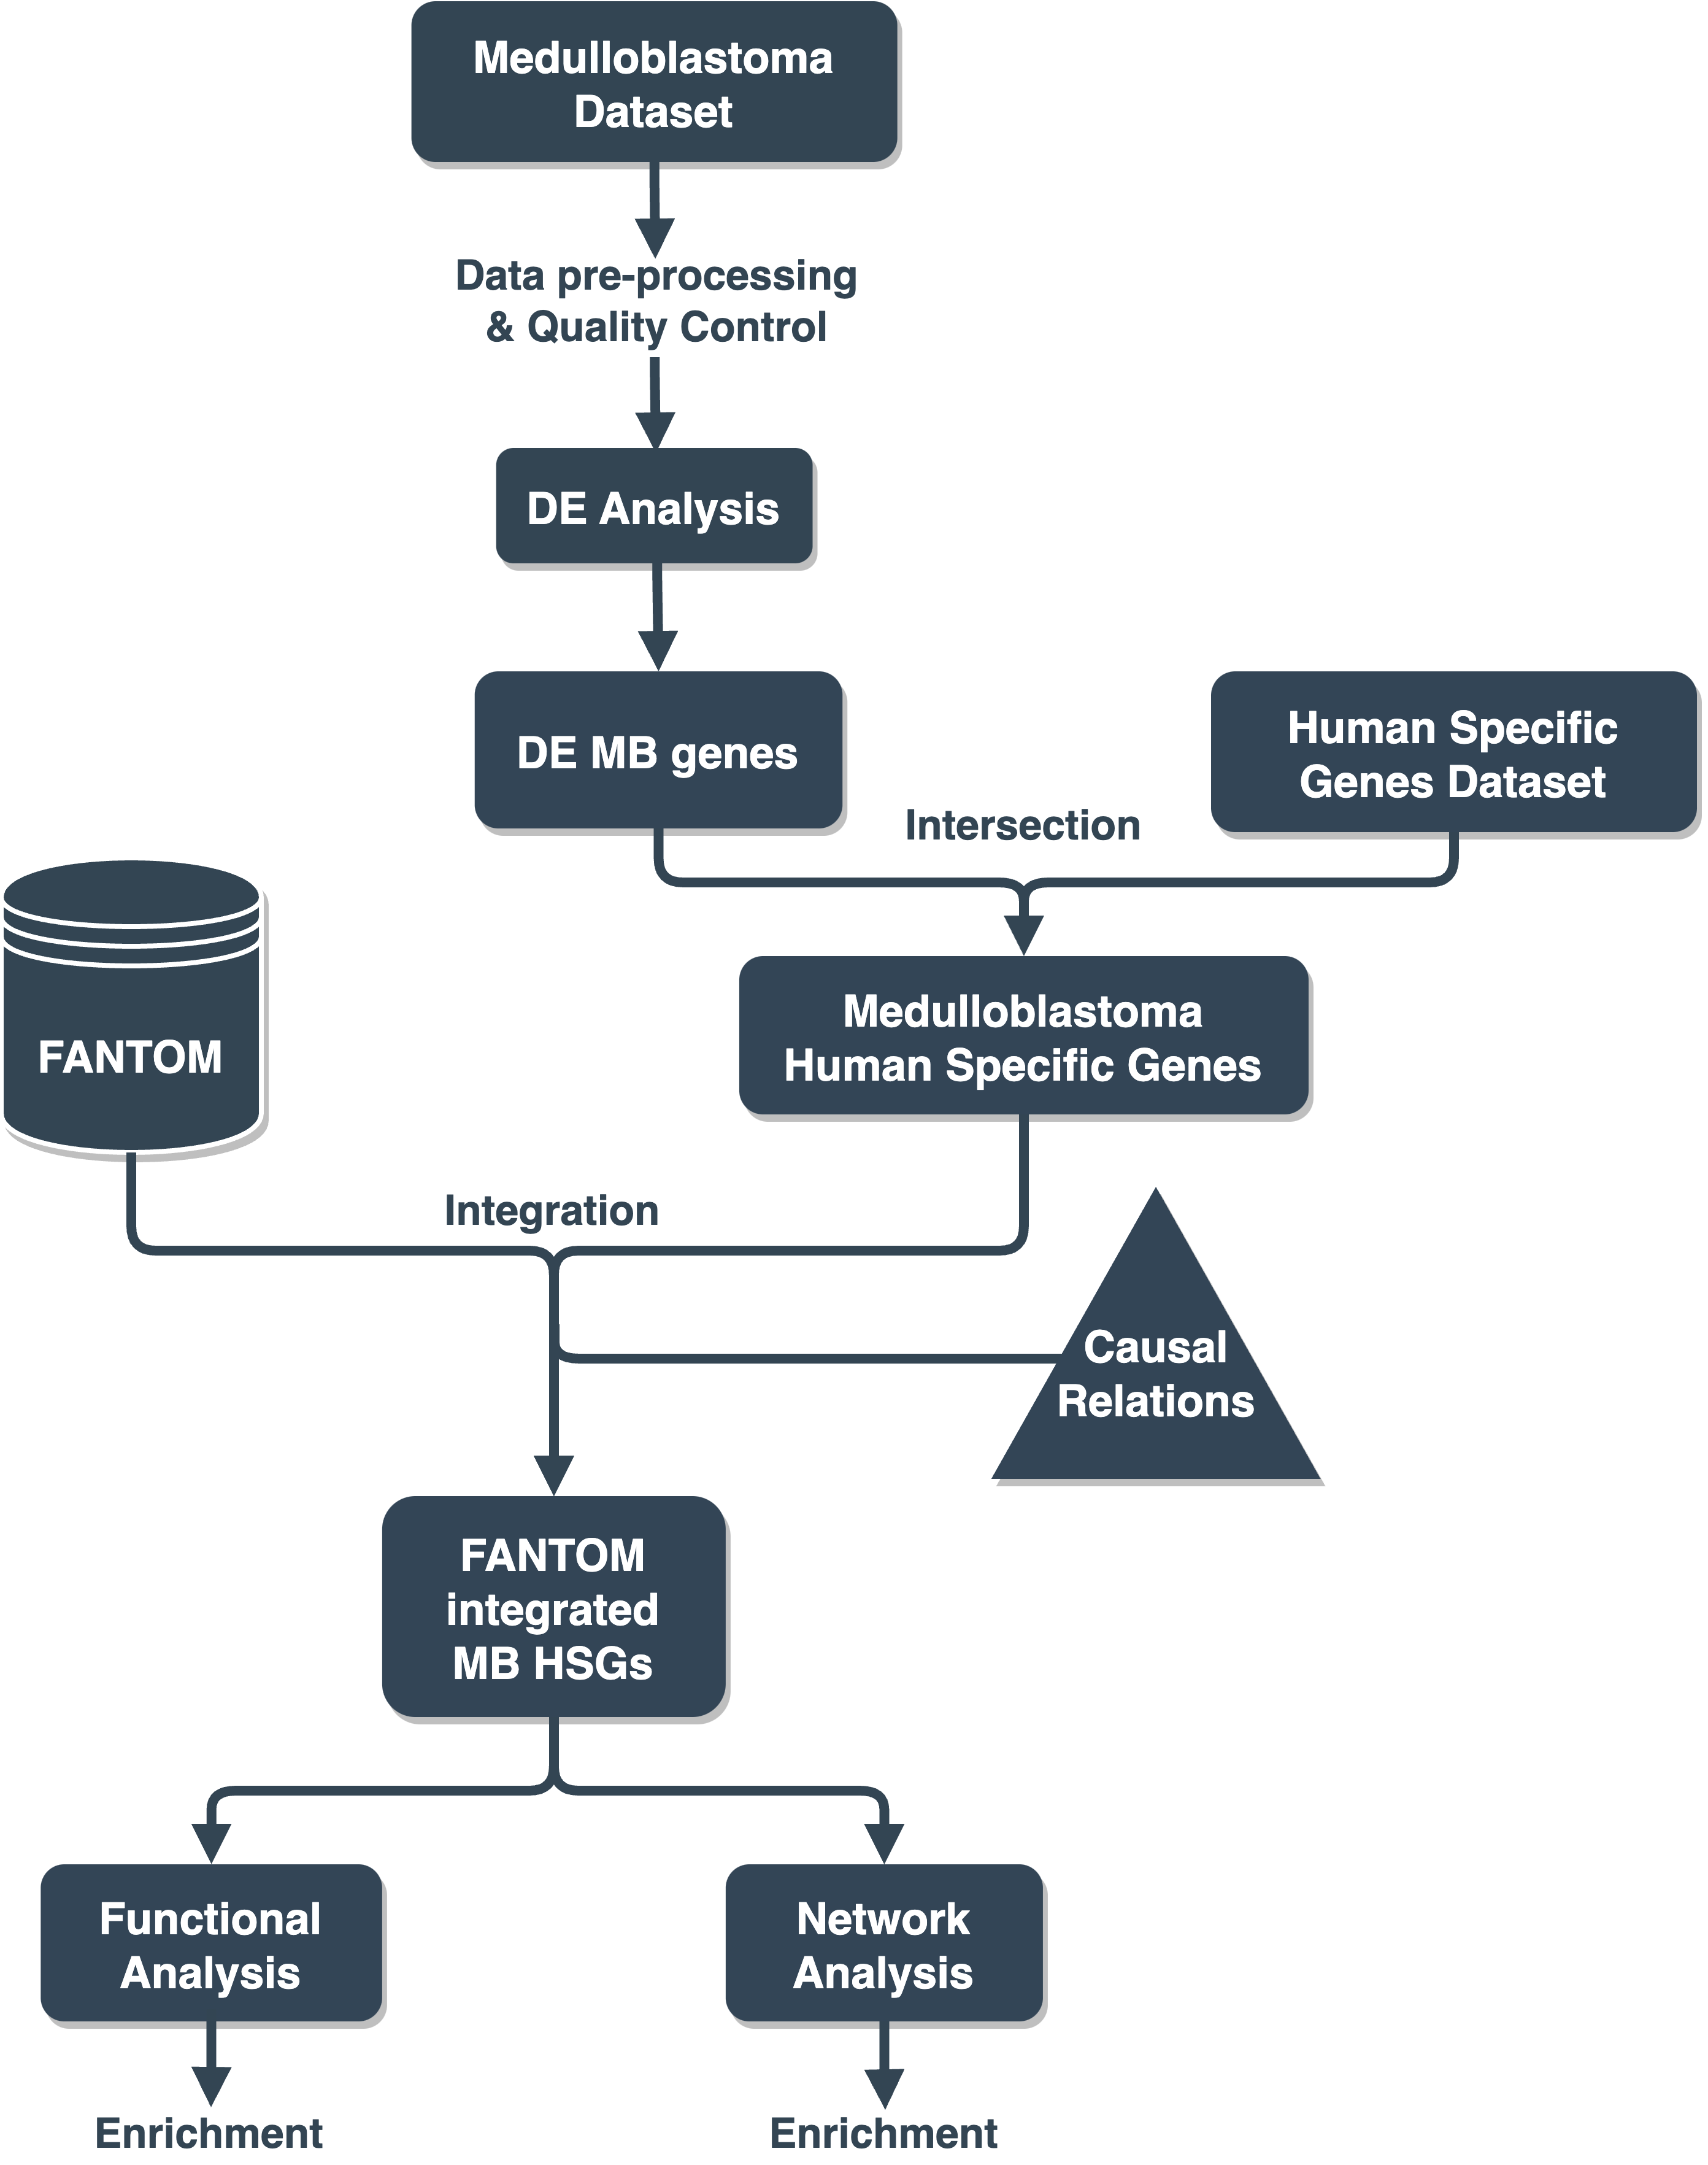
\includegraphics[width=0.45\textwidth]{project-proposal/figures/workflow.png}
    \caption{General workflow depicting the six main steps of the project.}
    \label{fig:workflow}    
\end{figure}

\section{Preliminary results}\label{sec:preliminary_results}
Through cBioPortal \cite{cbioportal}, we retrieved a list of genes that, due to mutations, are related to MB. By intersecting it with the list of HSGs \cite{bitar2019genes}, a set of 14 MB-related HSGs was obtained. \\
Using Cytoscape \cite{shannon2003cytoscape}, a network on the list of MB genes was built and MB-related HSGs were highlighted. We observed that 12 out of the 14 MB-related HSGs are taking part in many interactions \textbf{[\ref{fig:network}]}. This suggests us that it is worth analyzing in greater detail the possible contributions of HSGs in MB development.

\section{Expected results and contingency plans}\label{sec:expected_results}
By undertaking this analysis we expect to observe a functionally significant role played by Human Specific Genes with respect to non-HSGs. Should this functional significance be confirmed, further studies will be undertaken in order to evaluate the biological functions of the inferred genes. Otherwise, the absence of such functional significance could be as well considered a result. However, this would prompt us to possibly redirect our research focus towards another neurological disorder. 

\section{Project management}\label{sec:management}
Foremost the project will be developed in a teamwork driven manner. In the initial stages (e.g. data selection, data pre-processing, etc.), the entire team will work together. After integrating the MB HSGs with the FANTOM dataset \cite{fantom5}, the team will be ideally divided into two subgroups. The first one, consisting of Gaia Faggin and Huyen Pham, will be responsible for conducting the functional analysis. Meanwhile, the second subgroup, composed of Sara Baldinelli, Letizia De Pietri and Roan Spadazzi, will focus on network analysis. It is worth noting that both subgroups will maintain collaboration, allowing them to benefit from the diverse backgrounds and experiences of each member. Finally, the data interpretation and the conclusion will be discussed together.

\section{Resources}\label{sec:resources}
It is important to note that the resources listed are not to be considered final. As this is merely a project proposal, during the analysis phase, we may require additional libraries or tools.

\subsubsection*{\textit{Scanpy}}\label{sec:scanpy}
Since we are using scRNA-seq datasets, we will employ the \textit{Scanpy} library \cite{wolf2018scanpy}, a powerful Python tool tailored for the analysis of single-cell gene expression data. \textit{Scanpy} is purposefully designed in collaboration with \textit{anndata} \cite{virshup2021anndata}, encompassing a wide array of functionalities, including pre-processing, data visualization, clustering, trajectory inference, and differential expression analysis. 

\subsubsection*{\textit{NetworkX}}\label{sec:networkX}
To analyze the properties of the whole network we will use \textit{\textit{NetworkX}}, a Python package specifically designed for exploring and analyzing networks \cite{hagberg2008exploring}. \textit{NetworkX} offers a comprehensive set of tools for network representation, allowing nodes to be any hashable Python object and edges to contain diverse data. The package provides various data structures to handle different types of networks, along with a wide range of implemented algorithms for measuring network properties. 

\subsubsection*{Gene Ontology}\label{sec:gene_ontolgy}
Gene Ontology (GO) \cite{gene2019gene} is a comprehensive and widely-used bioinformatics resource that provides a standardized vocabulary and framework for describing the functions of genes and gene products. It categorizes genes into terms related to their molecular functions, biological processes, and cellular component, creating a structured, hierarchical system of annotations. 

\subsubsection*{Kyoto Encyclopedia of Genes and Genome}\label{sec:kegg}
The Kyoto Encyclopedia of Genes and Genome (KEGG) \cite{kanehisa2017kegg} is a broad and integrated bioinformatics database that serves as a valuable resource for understanding molecular-level information about biological pathways and functions. KEGG encompasses a wide range of data, including information on metabolic pathways, genetic sequences, diseases, and various other molecular processes. 

\subsubsection*{Cytoscape}\label{sec:cytoscape}
Cytoscape \cite{shannon2003cytoscape} is a powerful and widely-used bioinformatics software platform designed for the visualization and analysis of biological networks. It allows to create, manipulate, and explore complex network representations of biological data, such as protein-protein interactions, gene regulatory networks, and metabolic pathways. 

\subsubsection*{ggplot2}\label{ggplot2}
\textit{ggplot2} \cite{ggplot2} is a powerful plotting package designed for creating intricate visualizations from data stored in data frames. With its user-friendly commands, \textit{ggplot2} offers a programmable approach to specifying which variables to visualize, how they should be presented, and overall visual characteristics. It simplifies the process of generating complex plots and enhances the overall data visualization experience.






%----------------------------------------------------------------------------------------
%	REFERENCE LIST
%----------------------------------------------------------------------------------------
\phantomsection
\bibliographystyle{unsrt}
\bibliography{references.bib}

%----------------------------------------------------------------------------------------
%   SUPPLEMENTARY
%----------------------------------------------------------------------------------------

\newpage
\beginsupplement

\begin{sidewaysfigure*}[h!]
    \centering    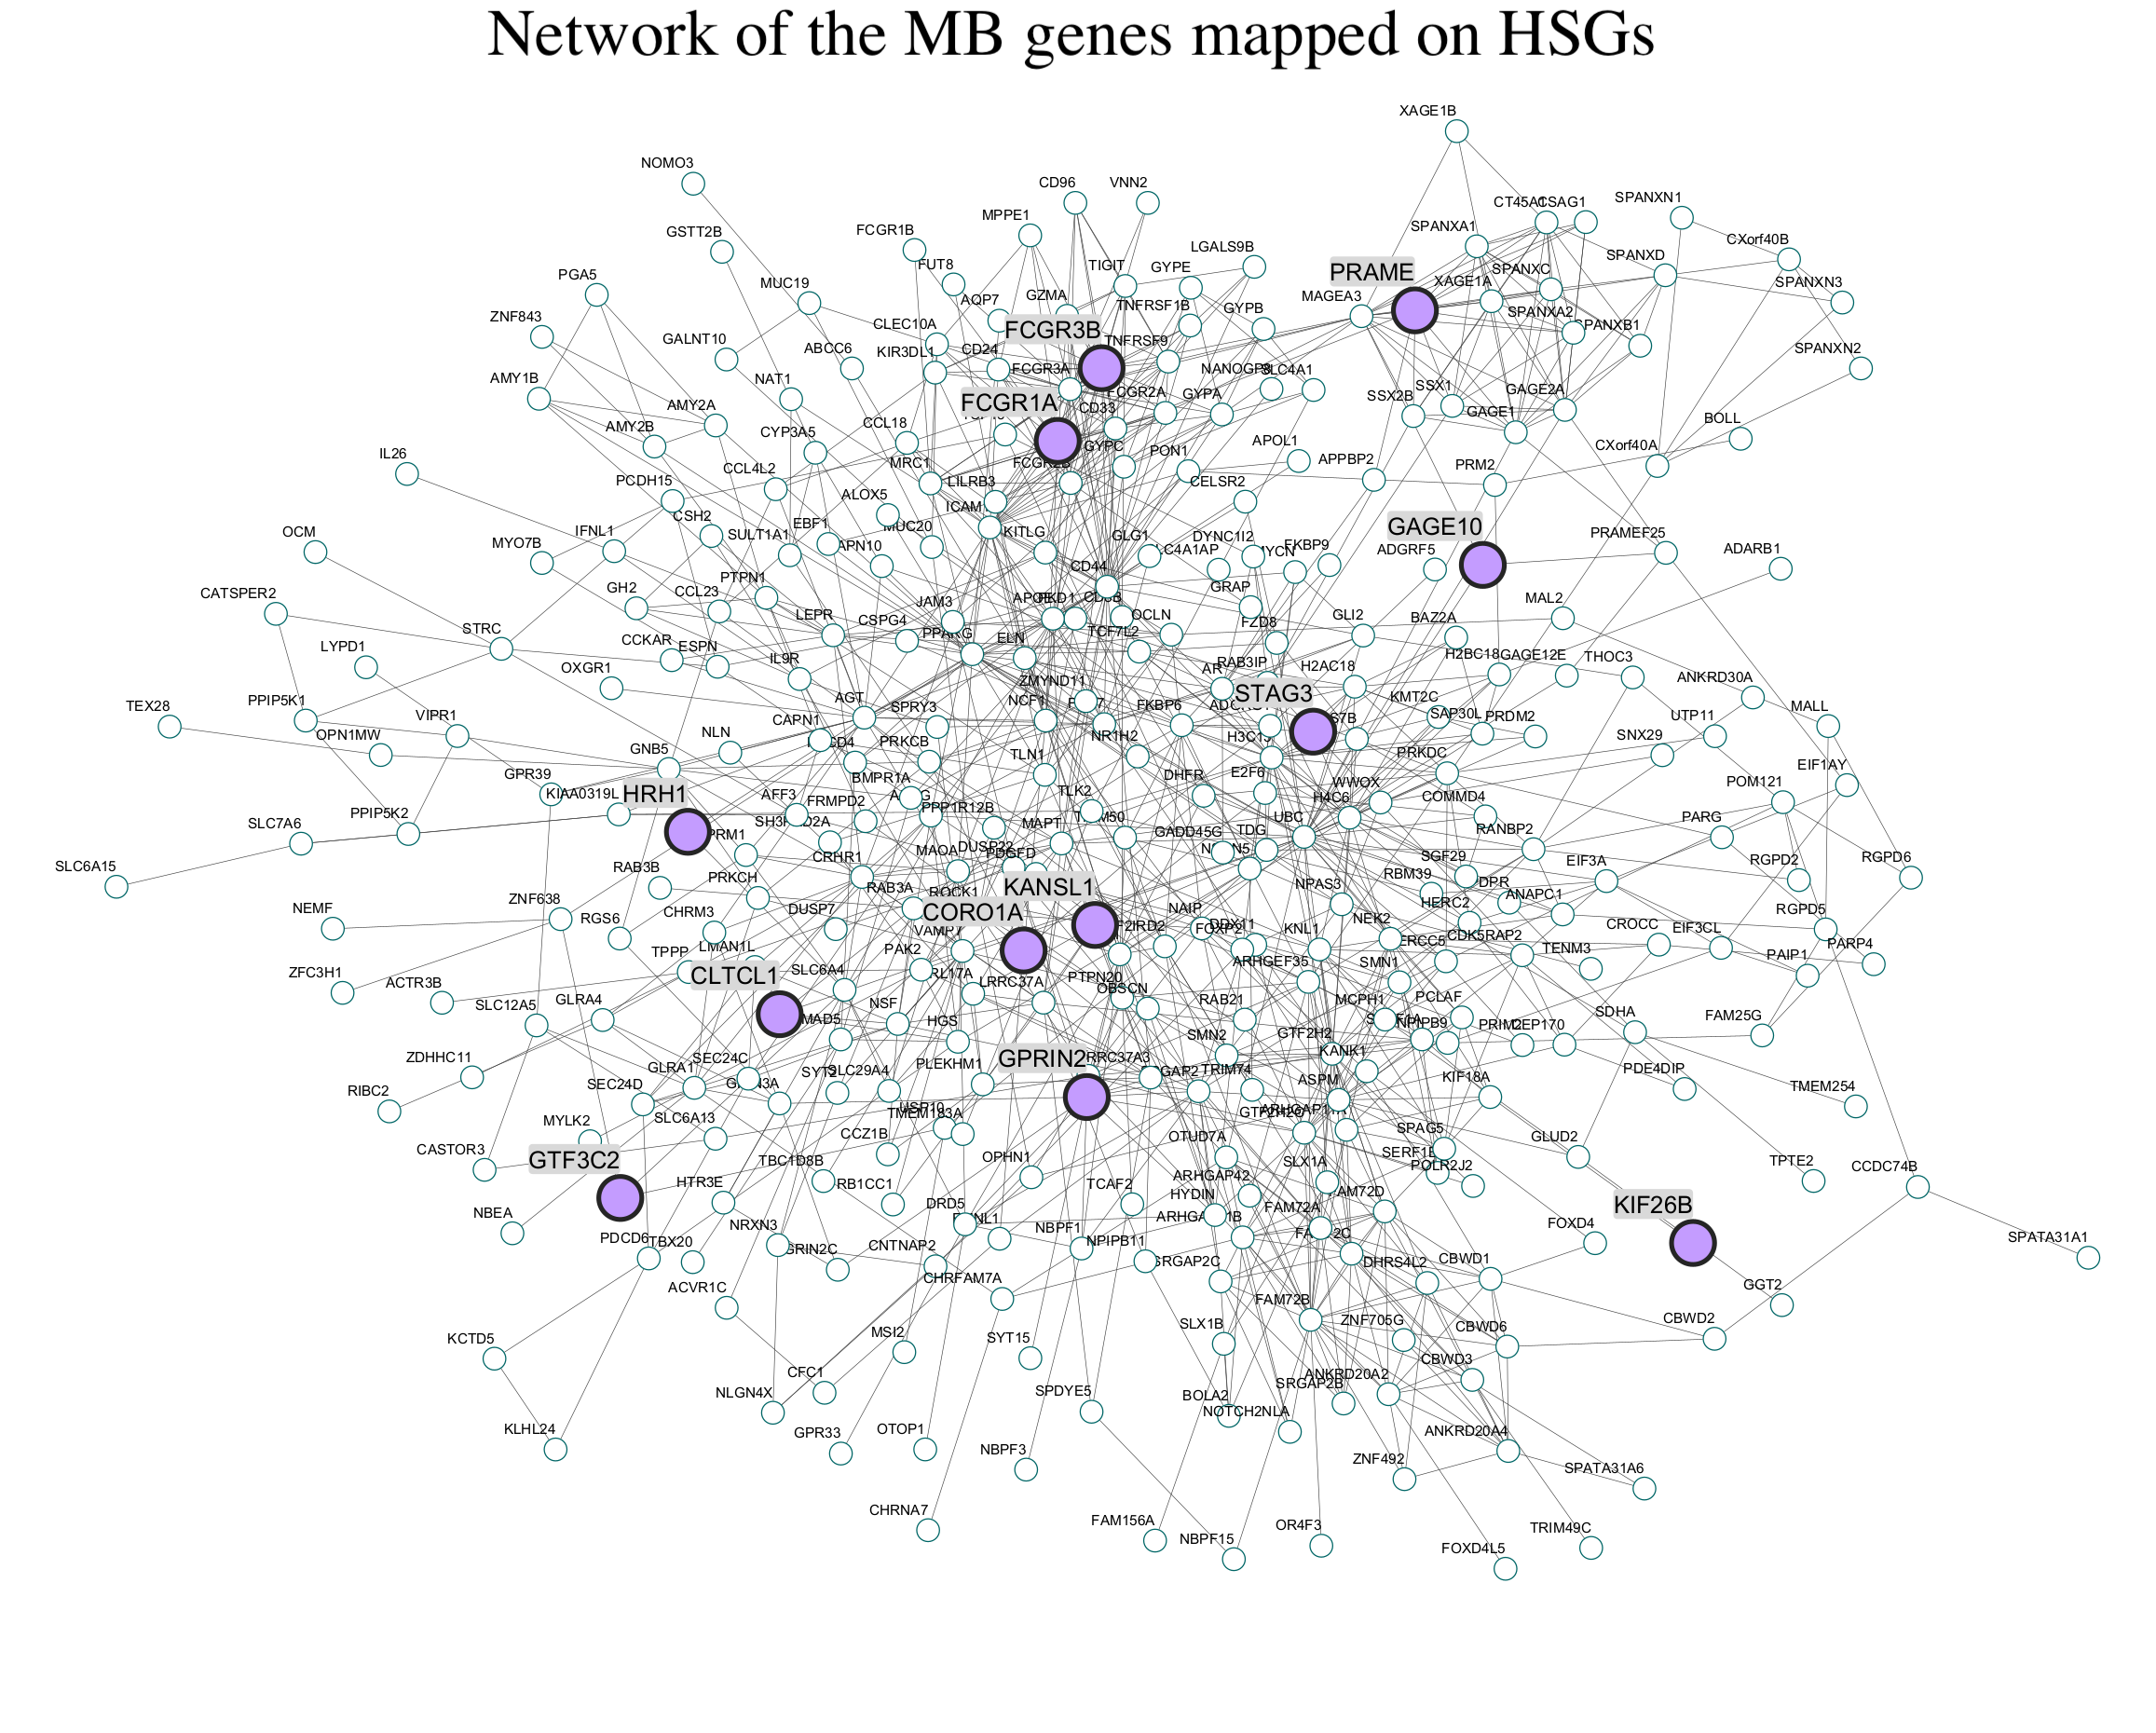
\includegraphics[width=1\textwidth]{project-proposal/figures/string_interactions_short.tsv2.png}
    \caption{}
    \label{fig:network}    
\end{sidewaysfigure*}




\end{document}
